\documentclass[12pt]{article} 
\usepackage[nohead]{geometry}
\usepackage[singlespacing]{setspace}
\usepackage[bottom]{footmisc}
\usepackage{indentfirst}
\usepackage{multirow}
\usepackage{amsmath, amssymb,amsfonts}
\usepackage{graphicx}
\usepackage[table]{xcolor}
\let\oldtabular\tabular 
\renewcommand{\tabular}{\large\oldtabular}
\usepackage{caption}
\usepackage{hyperref}
\hypersetup{
    pdftitle={FieldPaper},
    colorlinks=true,
    linkcolor=blue,
    filecolor=magenta,      
    urlcolor=cyan,
    citecolor=blue,
}
\urlstyle{same}
\usepackage{natbib}
\bibliographystyle{abbrvnat}
\setcitestyle{authoryear}
%\setlength\bibhang{0.5in}
\usepackage{float}

\newenvironment{proof}[1][Proof]{\noindent\textbf{#1.} }{\ \rule{0.5em}{0.5em}}
\newcommand{\pd}[2]{\frac{\partial#1}{\partial#2}}
\makeatletter
\def\@biblabel#1{\hspace*{-\labelsep}}
\makeatother
\geometry{left=1in,right=1in,top=1in,bottom=1in}


\title{Ethnic Enclaves and the Legacy of Internment}
\author{Dante Yasui}
\date{\today}

\begin{document}
\maketitle

\section{Intro}\label{intro}

\subsection{Research Question}\label{research-question}

\begin{itemize}

\item
  Did post-war relocation cause a permanent shift in the migration
  choices of Japanese Americans?
\end{itemize}

\begin{center}\rule{0.5\linewidth}{0.5pt}\end{center}

\subsection{Motivation}\label{motivation}

In the aftermath of Pearl Harbor over 100,000 Japanese Americans were subjected
to curfews, forced to assemble in temporary centers, and imprisoned in
internment camps from 1942 until the war's end. These families lost out on
years of earnings and education while also being forced to give up land and
belongings which they could not bring with them. The economic damages were
known to be large at the time, with the Japanese American Evacuation Claims Act
of 1948 leading to a total of \$148 million worth of claims on damage or lost
property and \$37 million actually being distributed
\citep{commission_on_wartime_relocation_personal_1983}. Because interned
families also left behind their records, it is very difficult to know the
actual value of lost property. However, there is modern causal evidence that
West Coast Japanese suffered higher rates of mortality lower long-term earnings
\citep{chin_longrun_2005}, \citep{saavedra_early_2013}, and less educational
attainment \citep{saavedra_school_2015} because of internment. 

\begin{figure}
    \centering
    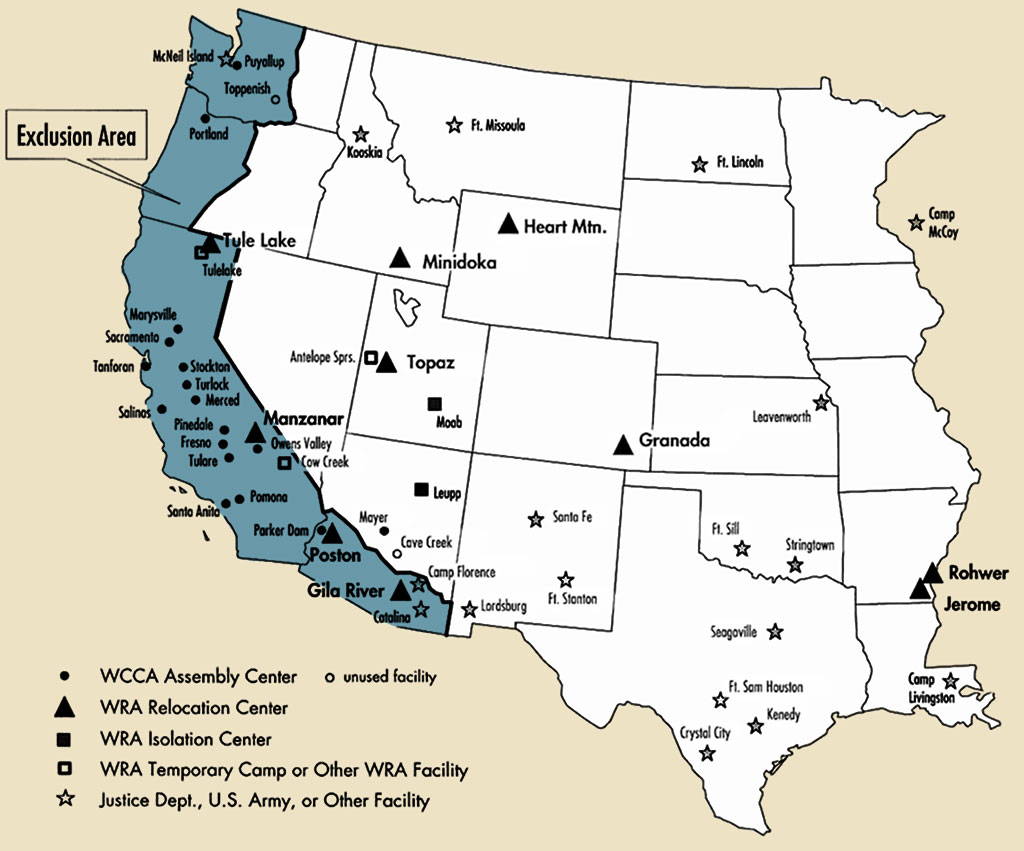
\includegraphics[width=.8\linewidth]{figures/PioCrtInternmentMap.jpg}
    \caption{Caption}
    \label{fig:internment_map}
\end{figure}

Aside from the importance of understanding the losses to internees, Japanese
Internment can also serve as an interesting natural experiment through the
involuntary nature of the experiences of internees. One question asked by
previous economic literature is the extent that locations in which people live
affect their economic outcomes such as upward mobility or earnings. It is
difficult to provide an unbiased causal estimate because households usually
have a large degree of choice in where they live. Previous studies have used a
variety of empirical strategies to separate out this causal effect including
controlling for observable characteristics like education
\cite{glaeser_cities_2001}, worker fixed-effects \citep{card_location_2021}, or
through leveraging other exogenous placements of households like the Moving to
Opportunity Experiment (\cite{ludwig_long-term_2013},
\cite{chetty_effects_2016}, etc). 

\begin{itemize}
\item
  Immigrant populations tend to concentrate near places of initial
  settlement
\item
  Integration/assimilation could be important for immigrant labor market
  outcomes

  \begin{itemize}
  
  \item
    \cite{damm_ethnic_2009}
  \end{itemize}
\item
  Evidence for Canadian Japanese internment having persistant effect on
  spatial Japanese distribution
\item
  \cite{chan_forced_2022}
\end{itemize}

\subsection{Initial Distribution of pre-war Japanese
Population}\label{initial-distribution-of-pre-war-japanese-population}

\begin{center}
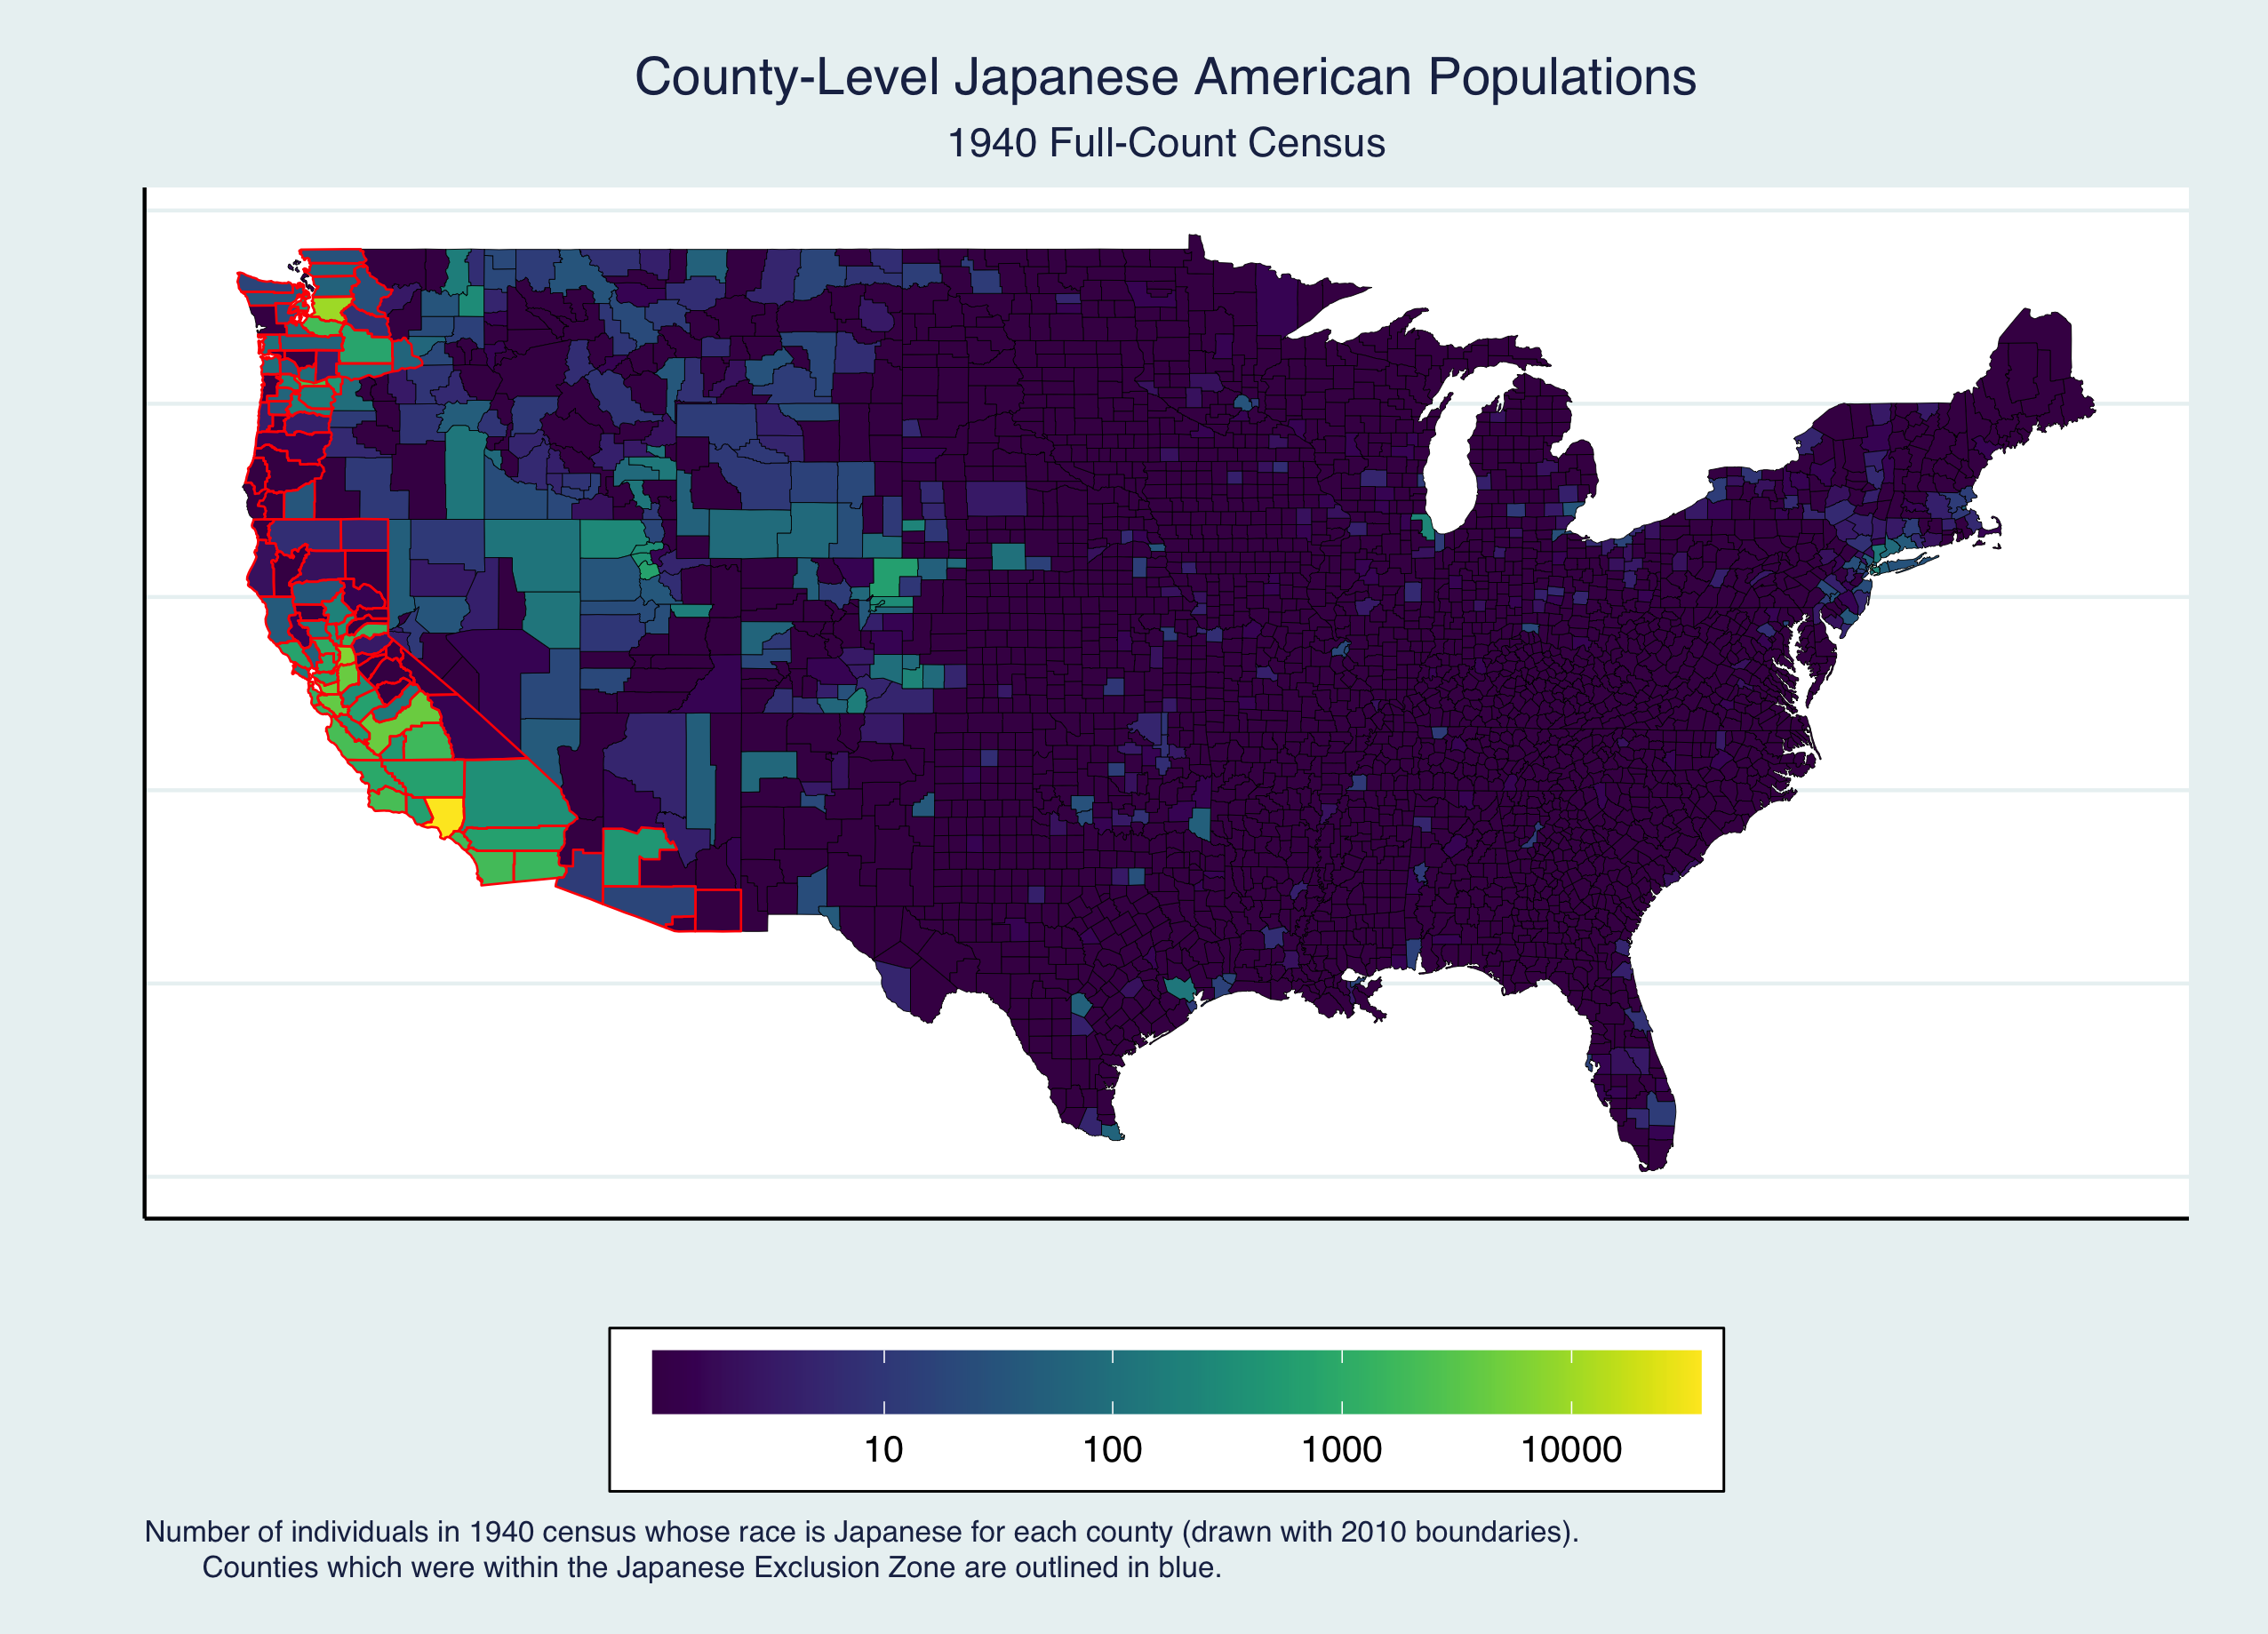
\includegraphics[width=1.0\textwidth]{figures/county_JAmap.png}
\end{center}

\subsection{Assignment of Internees to
Camps}\label{assignment-of-internees-to-camps}

\begin{center}
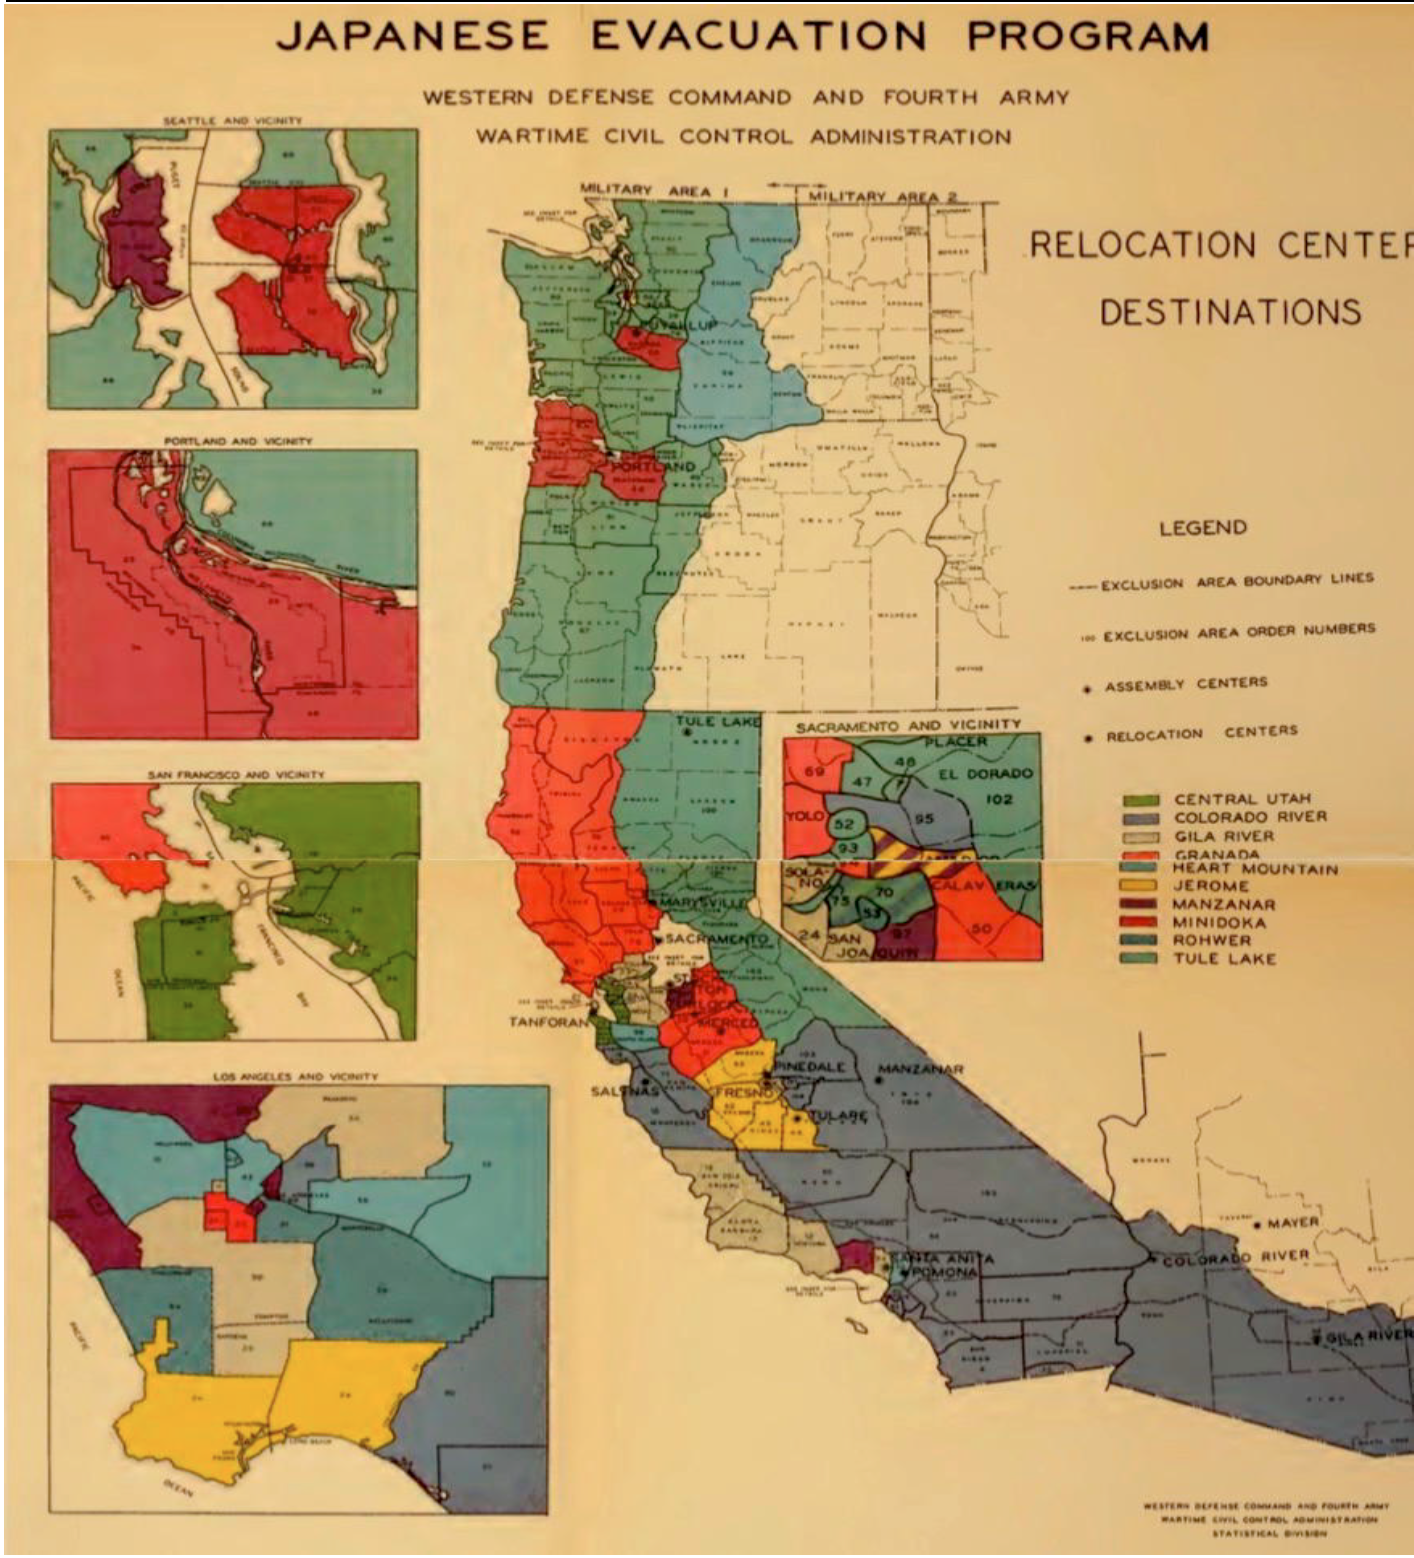
\includegraphics[width=.8\textwidth]{figures/WRAzonesmap.png}
\end{center}

\section{Data}\label{data}

I combine historical census data, geographical references, and archived internment camp records to create the final pooled cross-section of county-year-level observations that I use in my later analysis. 

\subsection{Population and Migration}\label{population-and-migration}

For long-run migration data, I use the Decennial Census data provided by
the US Census Bureau via the
\href{https://usa.ipums.org/usa/index.shtml}{Integrated Public Use
Microdata Series} \citep{ruggles_ipums_2024}. The census
samples for which county locations are available include the 1940, 1950,
1980, and 1990 1\% samples, the 1960 5\% sample, and the 1970 Form 2
Metro 1\% sample.

For the calculation of migration rates between counties, I define a
migrant as someone who reports that they either moved within the state,
between states, or that they were abroad five years ago (or in the past
1 year for 196l respondents). This excludes people who report moving
within the same house, didn't report their previous location, or when their
location was reported as unknown.

\subsection{Geography}\label{geography}

\subsubsection{Historical County Borders}\label{historical-county-borders}

Although most county borders did not change much in the second half of
the 20th Century, there were counties which split, merged, or had name
changes which can make cross-decade comparisons difficult. For these
reasons, I use the county boundaries as they appeared in the 1990 census.

% *** Maybe include figure to show some counties changing over time?

To standardize historical county-level data to 1990 county definitions, I implement the crosswalk
method by \cite{eckert_method_2020}. They overlay historical
county boundary shapefiles from \href{https://www.nhgis.org/}{NHGIS}
onto county boundaries for a specific target year (in this case 1990).
The sub-areas created by these overlays are used to calculate a set of
geographic weights which represent the fractions of a 1990 county's area
which were within the geographic areas of counties as they appear in
different decades (specifically the decades between and including 1940
to 1980). For my analysis, I take the crosswalk weights from the example
csv file for the end year 1990 which is published on the authors'
\href{https://github.com/liang-jack-a/EGLP_Crosswalk/tree/master}{github
repository}.

For the actual geographics boundaries of 1990 counties, I download the US county boundary shapefiles for the \href{https://www.census.gov/geographies/mapping-files/time-series/geo/tiger-line-file.html}{2008 TIGER/Line} basis from \url{nhgis.org} via the IPUMS NHGIS extract system.

I limit my data set to counties within the continental US, as Alaska and Hawaii were not yet states in 1940 and also because the effect of physical distance on migration is likely different for non-contiguous land areas.


\subsubsection{Camp Locations}\label{camp-locations}

Locations for historical interment camp locations were originally archived by
\href{http://encyclopedia.densho.org/War_Relocation_Authority/\#Planning_the_Camps}{Densho
Encyclopedia} and I downloaded these records in csv form via the
\href{https://www.arcgis.com/home/item.html?id=69183af8d45d4f46a9dc4eba99440891}{Behind
Barbed Wires} story project's website
(\cite{chrkan_behind_2019}, \cite{robinson_war_2023}).

I use the \texttt{sf} package in \texttt{R} to georeference the latitude-longitude coordinates from these records and project them to the same Coordinate Reference System used for the NHGIS shapefiles \citep{pebesma_simple_2018}.
\footnote{NHGIS uses the Contiguous Albers Equal Area Conic projection.}
This allows me to use the \texttt{st\_distance} function to obtain the distance matrix between all county-camp pairs and then select the closest camp to each county and the associated distance for my main independent variable.

\begin{figure}[H]
    \centering
    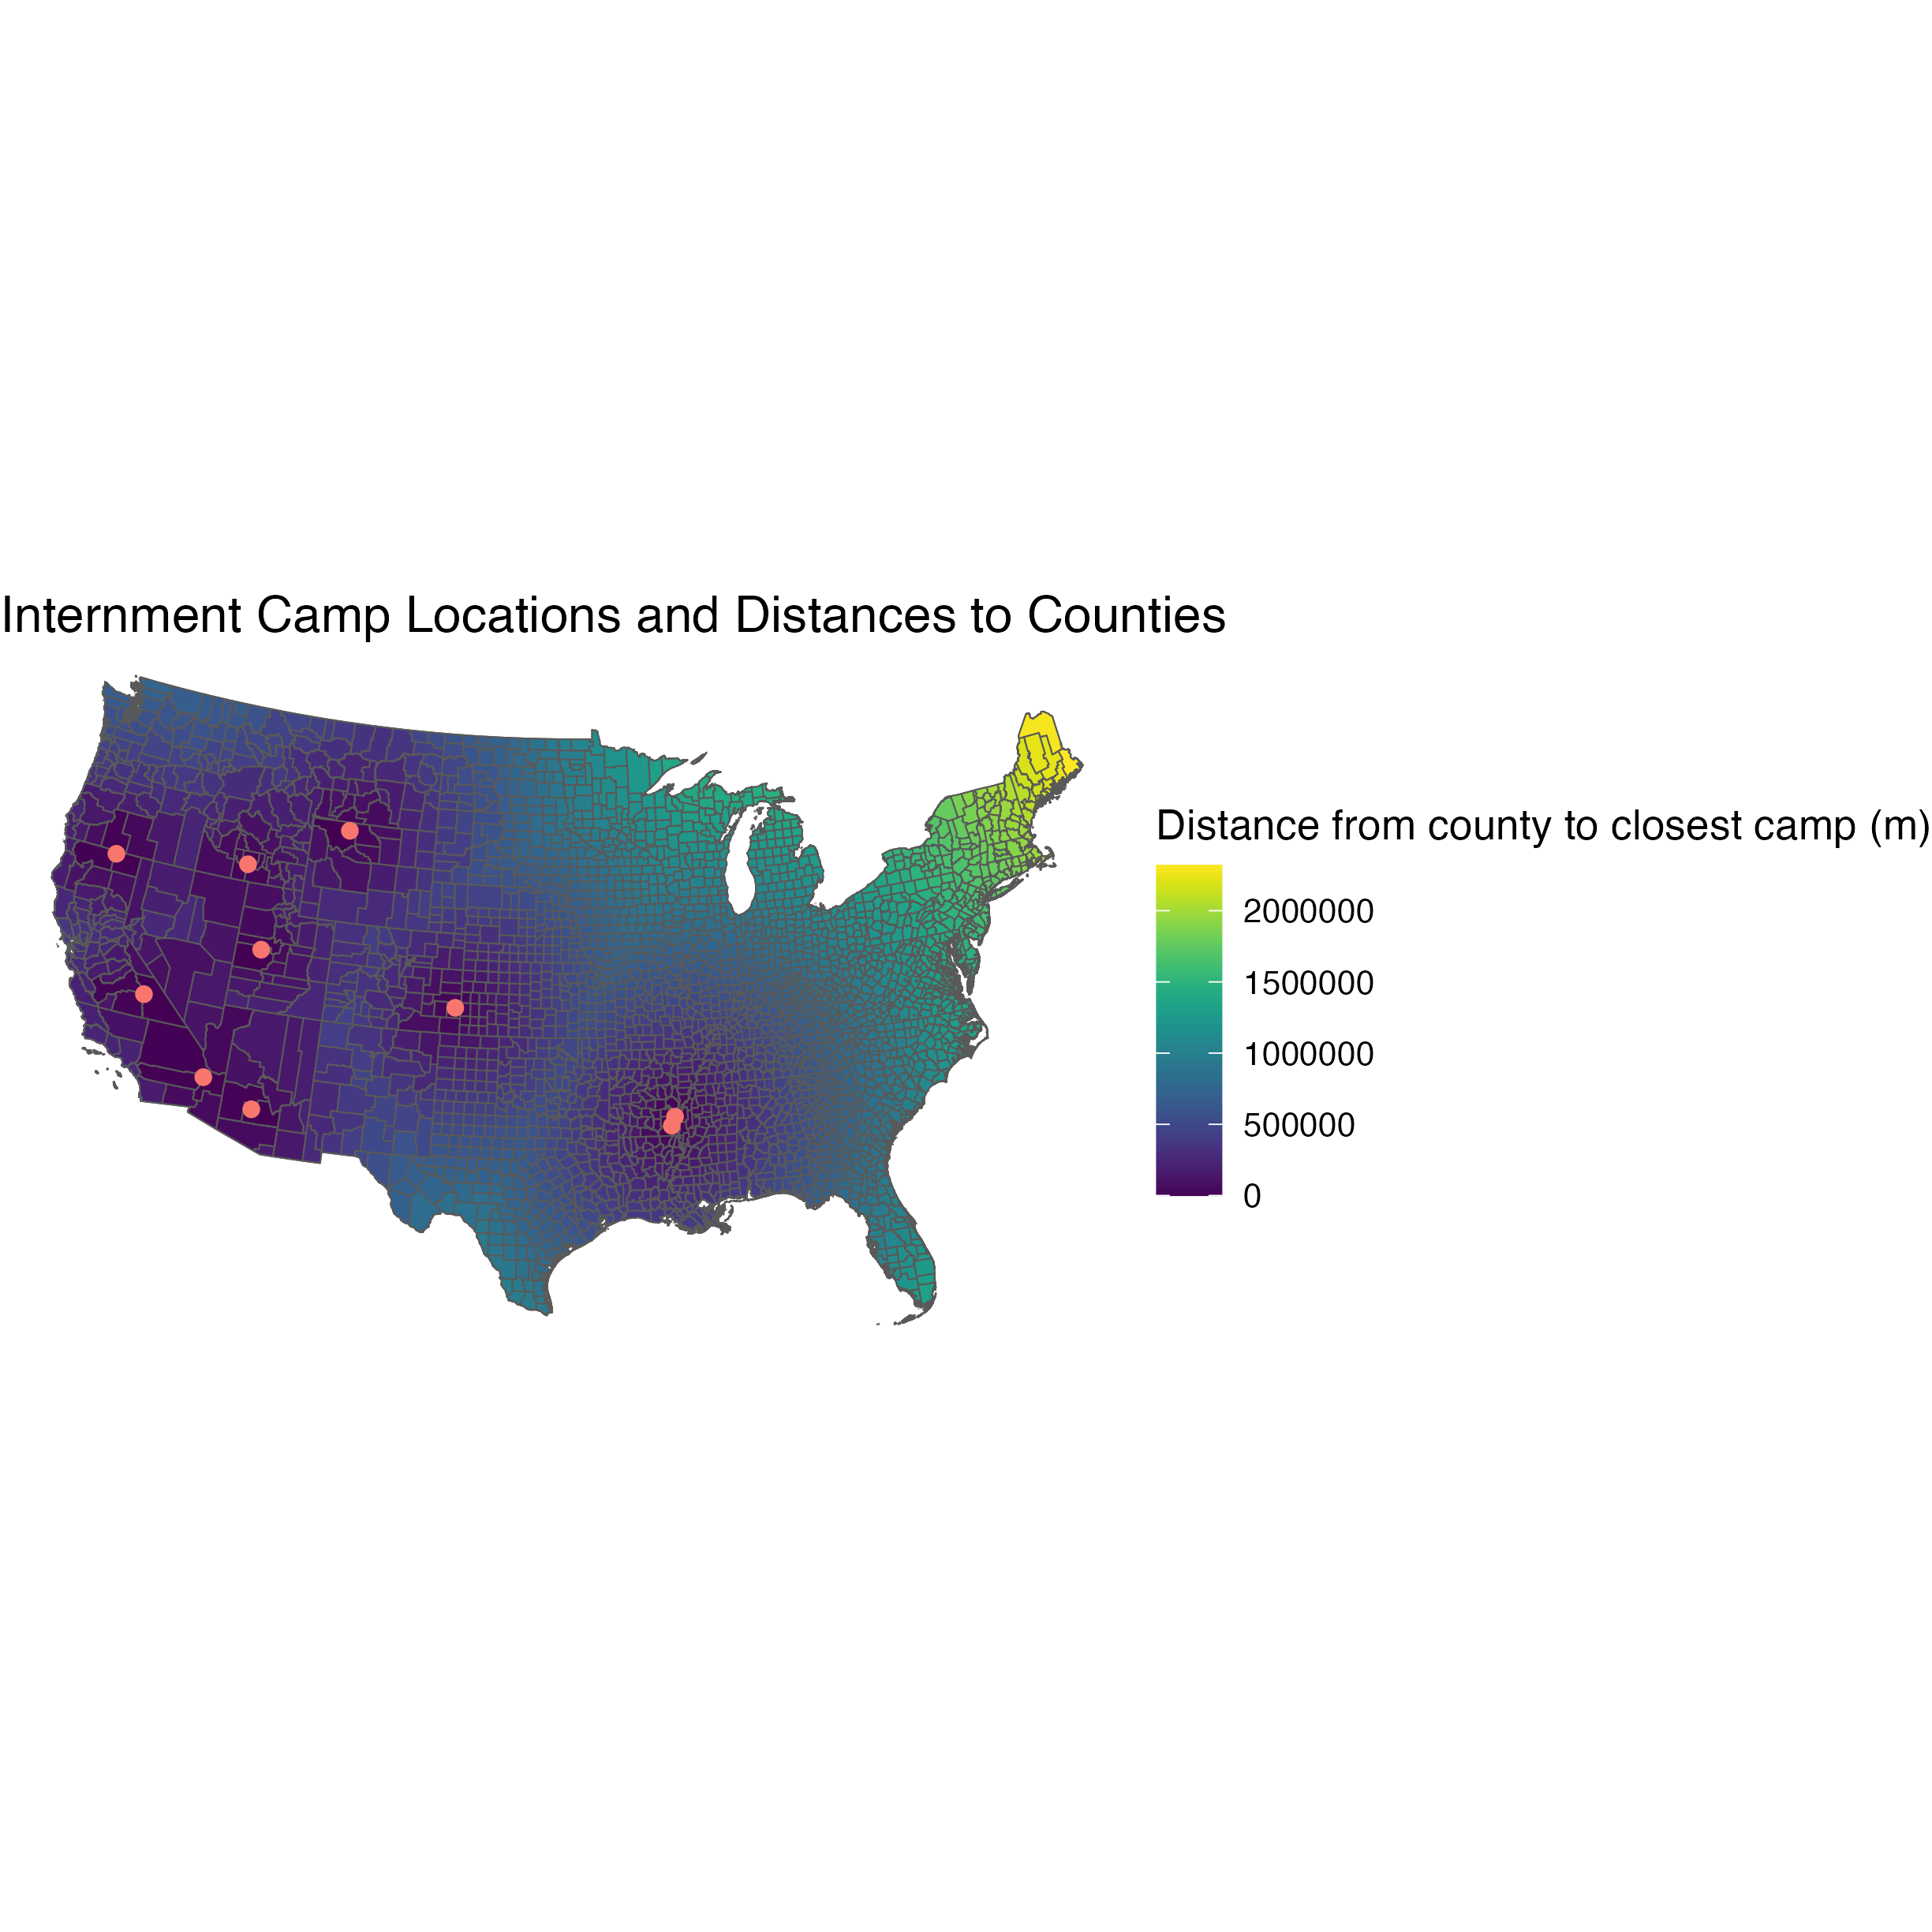
\includegraphics[width=1.0\textwidth]{figures/countymap.png}
    \caption{WRA internment camp locations with 1990 counties and their distances to each camp}
    \label{fig:countymap}
\end{figure}

Figure \ref{fig:countymap} shows the relationship between the internment camp locations and county boundaries. 
Each of the red dots represents the historical location of one of the ten WRA internment camps. 
From West to East they are:
Tule Lake and Manzanar, California;
Gila River, Arizona;
Minidoka, Idaho;
Topaz, Utah;
Heart Mountain, Wyoming,
Amache, Colorado;
and
Jerome and Rohwer, Arkansas.

\subsection{Historical counties
dataset}\label{historical-counties-dataset}

% Table created by stargazer v.5.2.3 by Marek Hlavac, Social Policy Institute. E-mail: marek.hlavac at gmail.com
% Date and time: Wed, Sep 18, 2024 - 16:34:32
\begin{table}[!h] \centering 
  \caption{County-Year Summary Statistics} 
  \label{ctysumstats} 
\begin{tabular}{@{\extracolsep{5pt}}lccccc} 
\\[-1.8ex]\hline 
\hline \\[-1.8ex] 
Statistic & \multicolumn{1}{c}{N} & \multicolumn{1}{c}{Mean} & \multicolumn{1}{c}{St. Dev.} & \multicolumn{1}{c}{Min} & \multicolumn{1}{c}{Max} \\ 
\hline \\[-1.8ex] 
Population & 4,257 & 132,663 & 356,496 & 0 & 7,495,400 \\ 
New Migrants & 4,257 & 53,316 & 148,182 & 0 & 3,216,300 \\ 
Migrant/Pop Ratio & 4,257 & 0.47 & 0.16 & 0.00 & 1.47 \\ 
New Japanese American Migrants & 877 & 720 & 3,199 & 0 & 60,480 \\ 
Current Japanese Population & 877 & 2,036 & 10,507 & 0 & 191,000 \\ 
Japanese/Total Migration Ratio & 877 & 0.0043 & 0.0173 & 0.00 & 0.34 \\ 
Average Age & 4,257 & 29.85 & 5.69 & 0.00 & 63.92 \\ 
Percent Female & 4,257 & 0.48 & 0.08 & 0.00 & 1.00 \\ 
Average Wage & 4,257 & 1,824.29 & 3,819.30 & 0.00 & 25,127.07 \\ 
Unemployment Rate & 4,257 & 0.07 & 0.05 & 0.00 & 1.00 \\ 
Distance to Closest Camp & 4,252 & 779,219 & 466,578 & 0 & 2,318,914\\ 
\hline \\[-1.8ex] 
\end{tabular} 
\end{table} 


After narrowing down to counties which can be observed in each census
year and then translating the historical counties to 1990 county
boundaries, I am left with 3082 counties with observable migration rates
in 1940, 108 in 1950, 410 in 1960, 115 in 1970, 254 in 1980, and 290 in
1990.

My primary dataset is therefore a pooled-crossection with a total number
of 4,257 county-year level observations. Each observation represents an
individual county at a given year in time if it had the same borders as
it had in 1990.

The Census Bureau confidentiality standards state that public-use
microdata will cannot show report locations with populations of less
than 100,000 people. For this reason, many sparsely-populated counties
will be omitted from my sample because there are not enough observations
for the Census to report locations of individuals living there.

All county-level observations in my final dataset are created by first taking the weighted average of each variable across all individuals who have an identifiable address within any county 

\phantomsection\label{cell-fig-comparesamplepops}
\begin{figure}[H]
\centering{
 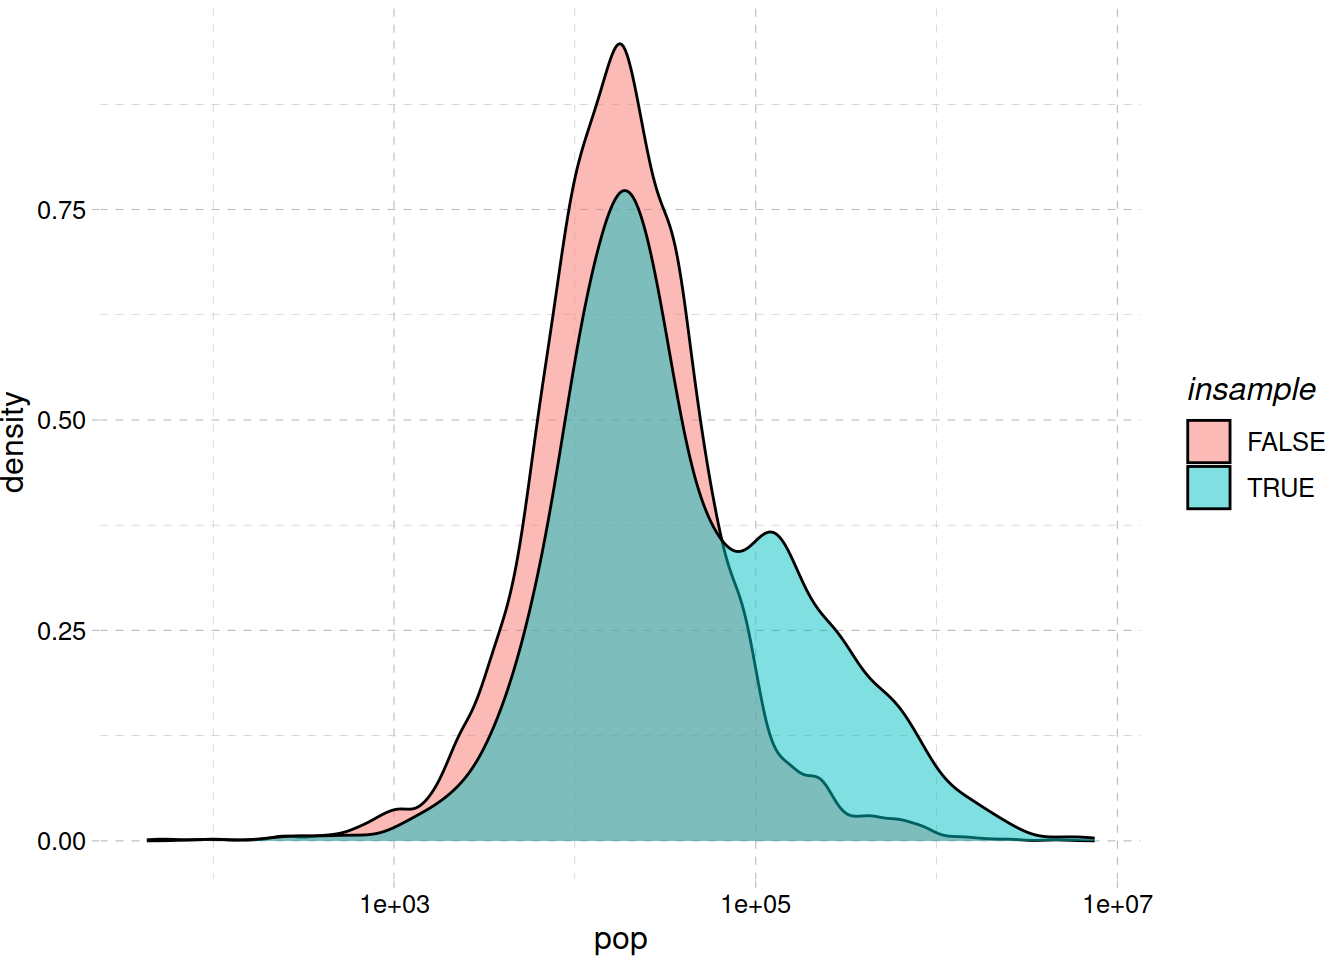
\includegraphics[width=.8\textwidth]{figures/fig-comparesamplepops-1.png}
}
\caption{\label{fig-comparesamplepops}County-year level population
distributions for identifiable (insample = TRUE) and for counties which are not in the final sample (insample = FALSE)}
\end{figure}%

The average population of the census-year observations in my sample is
133,000 while the average population for
crosswalked census-year observations outside my sample is
3,930,000. The fact that my sample is not
fully representative of all county sizes will be a challenge for the
external validity of my findings to extrapolate my results to smaller
counties for which I have less information on. However,
Figure~\ref{fig-comparesamplepops} shows that two different densities of
county-year populations observed in and out of the main sample have
similar shapes with the exception of a larger right-tail in the
in-sample density plot. This reflects the fact that counties with
populations of greater than 100,000 meet the Census Bureau's
confidentiality criteria, while data from smaller counties are subject
to stricter confidentiality measures.


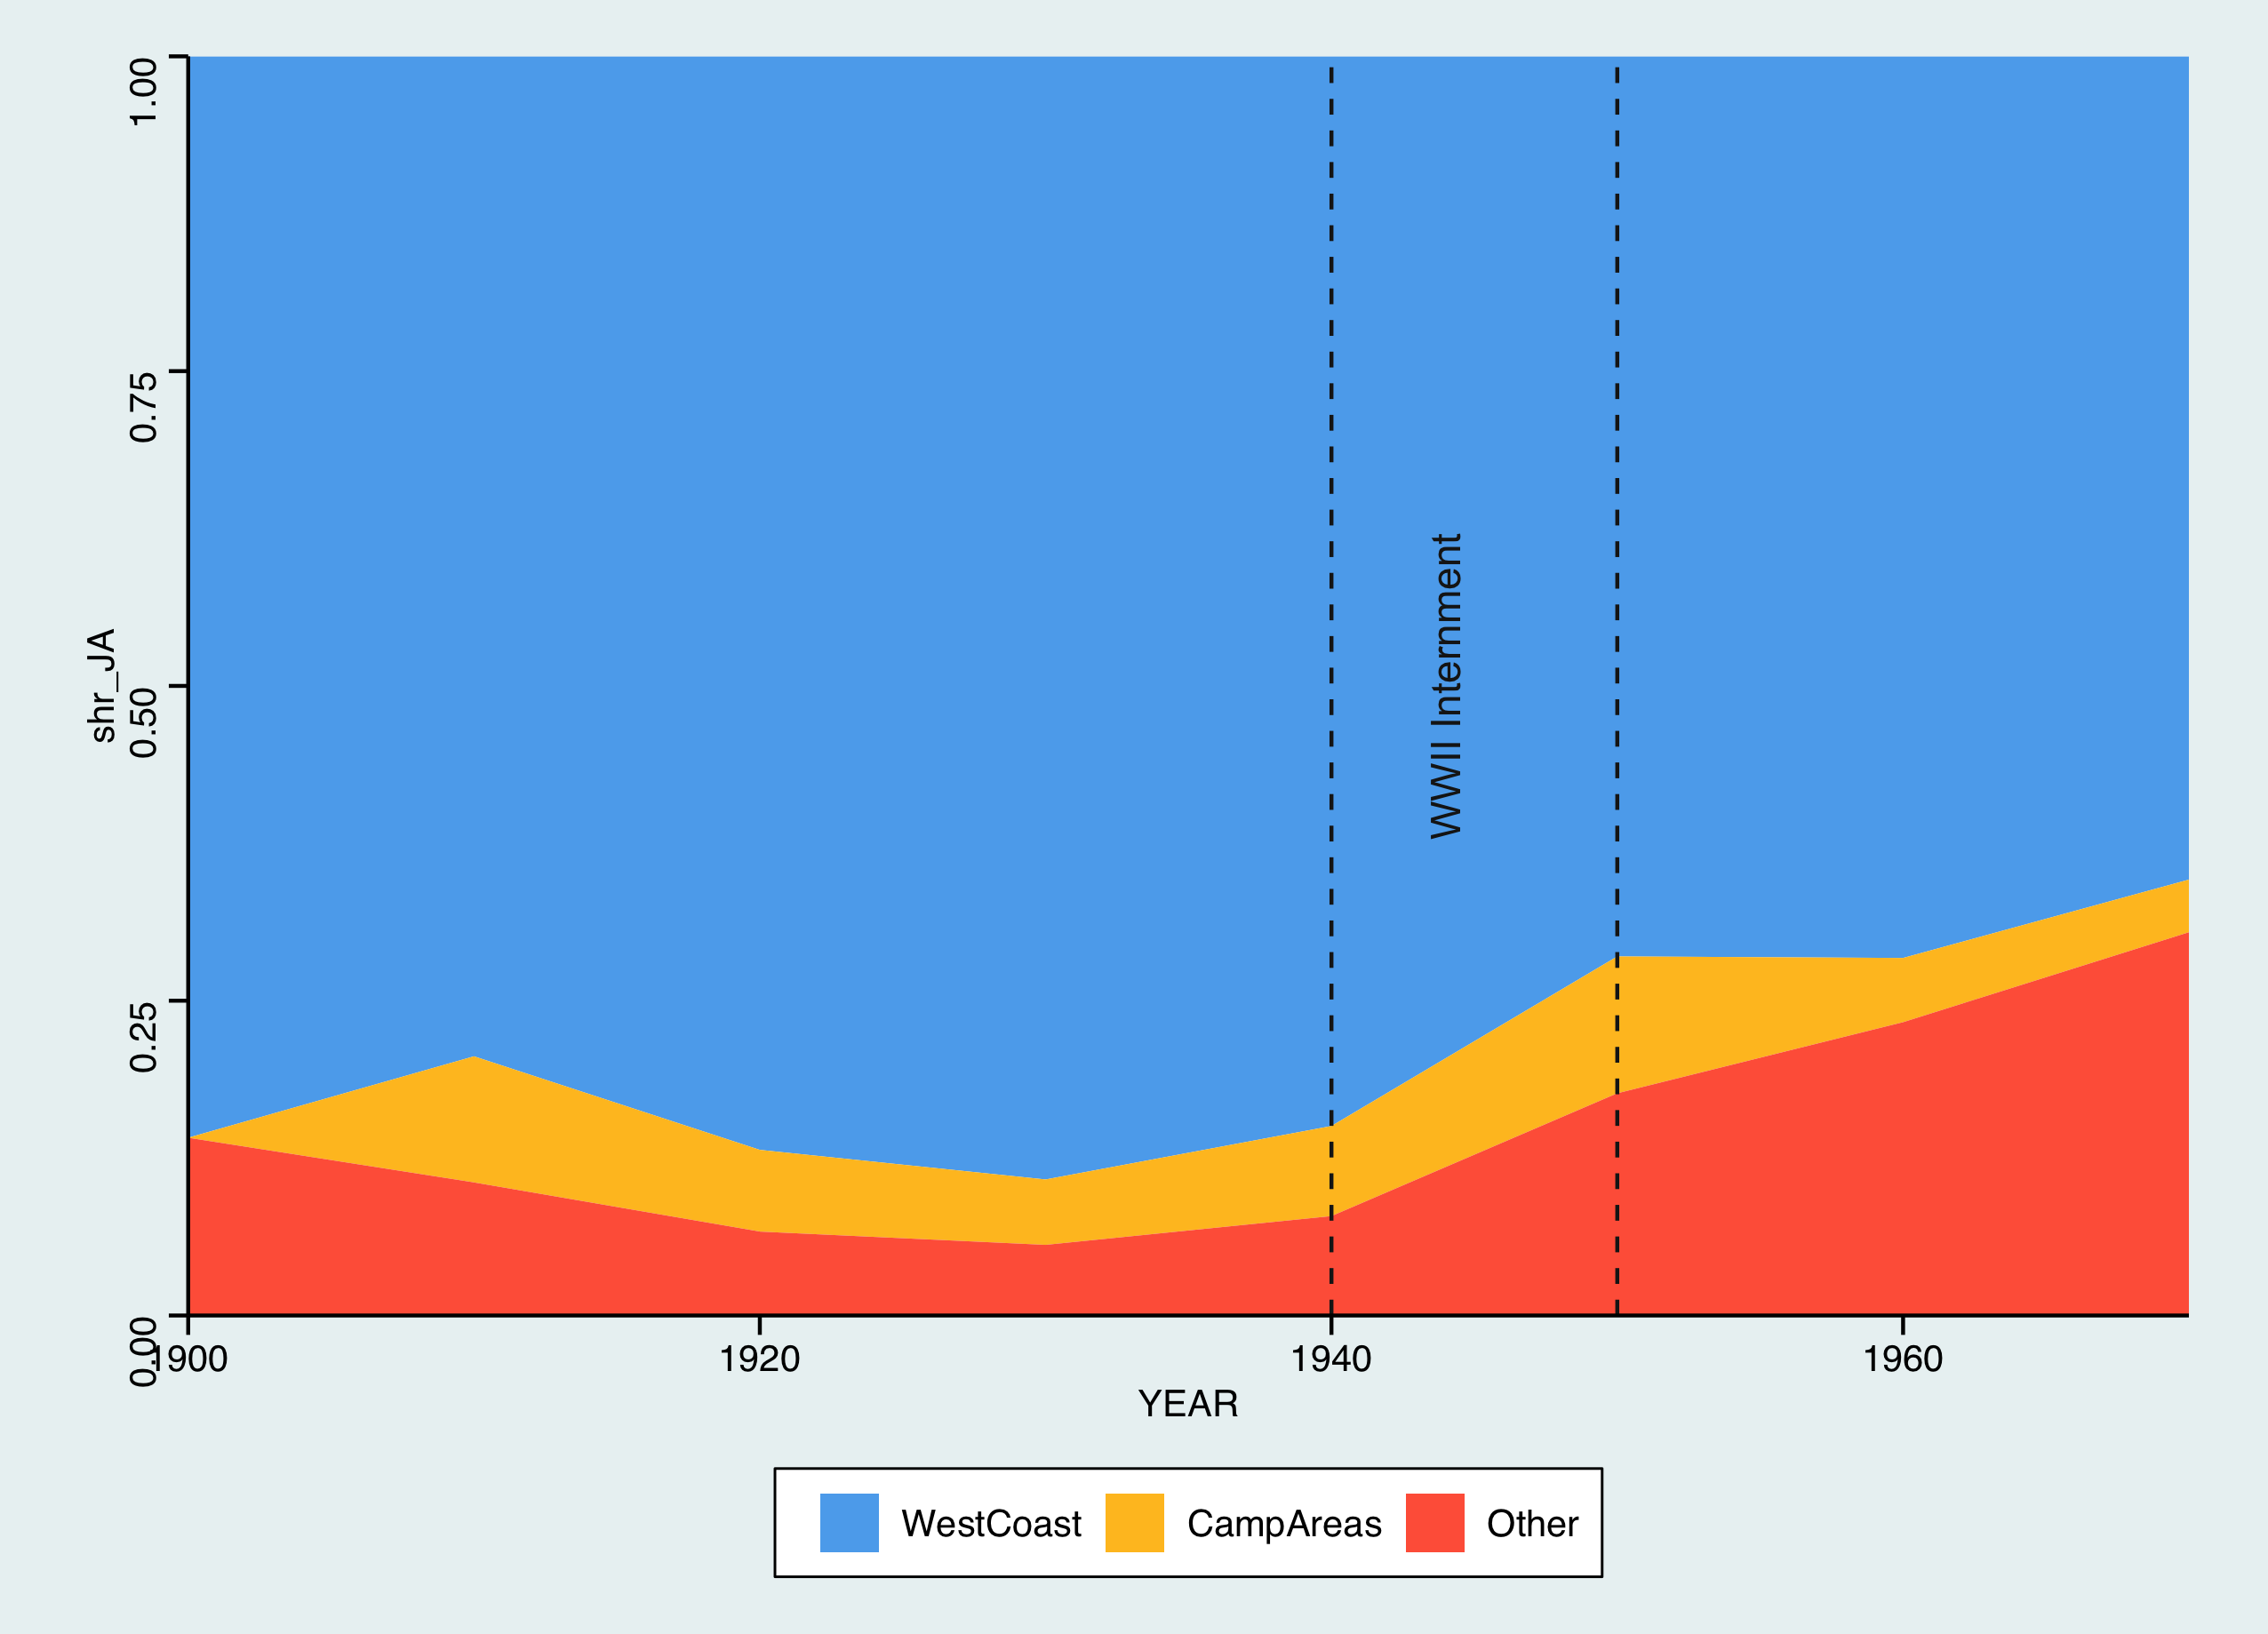
\includegraphics[width=1.0\textwidth]{figures/shareareaplot.png}

\subsection{NHGIS geo}\label{nhgis-geo}

\section{Methods}\label{methods}

\subsection{immigration on dist to
camps}\label{immigration-on-dist-to-camps}

\begin{equation}
    \frac{mig\_japn_{it}}{mig\_total_{it}} = \beta_0 + \beta_1 \min_{c\in C} Dist^{c\rightarrow i} 
+ \mathbb{X}_{ct} \gamma +  \epsilon_{ct}
\end{equation}

\subsubsection{within cont. US migration of japanese
americans}\label{within-cont.-us-migration-of-japanese-americans}

\subsubsection{new immigration from
japan}\label{new-immigration-from-japan}

\subsection{individual-level characteristics vs
internees?}\label{individual-level-characteristics-vs-internees}

\section{Results}\label{results}


% Table created by stargazer v.5.2.3 by Marek Hlavac, Social Policy Institute. E-mail: marek.hlavac at gmail.com
% Date and time: Wed, Sep 11, 2024 - 17:28:07
\begin{table}[!htbp] \centering 
  \caption{Effects of Distance to Closest Camp on Japanese Migration by Decade} 
  \label{} 
\begin{tabular}{@{\extracolsep{5pt}}lcccccc} 
\\[-1.8ex]\hline 
\hline \\[-1.8ex] 
 & \multicolumn{6}{c}{\textit{Dependent variable:}} \\ 
\cline{2-7} 
\\[-1.8ex] & \multicolumn{6}{c}{Ratio of Japanese American migrants to total migrants} \\ 
 & 1940 & 1950 & 1960 & 1970 & 1980 & 1990 \\ 
\\[-1.8ex] & (1) & (2) & (3) & (4) & (5) & (6)\\ 
\hline \\[-1.8ex] 
 log(campclosest\_dist) & 0.096 & 0.032 & $-$0.024 & $-$0.085 & $-$0.059 & $-$0.120 \\ 
  & (0.076) & (0.074) & (0.084) & (0.077) & (0.079) & (0.081) \\ 
  Constant & $-$1.237 & $-$0.319 & 0.506 & 1.367 & 1.011 & 1.895 \\ 
  & (1.099) & (1.061) & (1.210) & (1.113) & (1.139) & (1.172) \\ 
 \hline \\[-1.8ex] 
Observations & 548 & 553 & 499 & 512 & 492 & 537 \\ 
R$^{2}$ & 0.003 & 0.0004 & 0.0002 & 0.002 & 0.001 & 0.004 \\ 
Adjusted R$^{2}$ & 0.001 & $-$0.001 & $-$0.002 & 0.0004 & $-$0.001 & 0.002 \\ 
\hline 
\hline \\[-1.8ex] 
\textit{Note:}  & \multicolumn{6}{r}{$^{*}$p$<$0.1; $^{**}$p$<$0.05; $^{***}$p$<$0.01} \\ 
\end{tabular} 
\end{table} 



% Table created by stargazer v.5.2.3 by Marek Hlavac, Social Policy Institute. E-mail: marek.hlavac at gmail.com
% Date and time: Mon, Sep 16, 2024 - 16:07:49
\begin{table}[!htbp] \centering 
  \caption{Effects of Distance to Closest Camp on Japanese Migration by Decade} 
  \label{ezdistreg} 
\begin{tabular}{@{\extracolsep{2pt}}lcccccc} 
\\[-1.8ex]\hline 
\hline \\[-1.8ex] 
 & \multicolumn{6}{c}{\textit{Dependent variable:}} \\ 
\cline{2-7} 
\\[-1.8ex] & \multicolumn{6}{c}{Ratio of Japanese American migrants to total migrants} \\ 
 & 1940 & 1950 & 1960 & 1970 & 1980 & 1990 \\ 
\\[-1.8ex] & (1) & (2) & (3) & (4) & (5) & (6)\\ 
\hline \\[-1.8ex] 
 Log(Distance) & $-$1.247$^{***}$ & 0.003 & $-$0.088$^{***}$ & $-$0.157$^{***}$ & $-$0.046 & $-$0.071$^{*}$ \\ 
  & (0.417) & (0.393) & (0.026) & (0.053) & (0.065) & (0.038) \\ 
  Evac. Zone (EZ) & $-$20.488$^{**}$ & $-$3.536 & $-$2.128$^{***}$ & $-$4.701$^{***}$ & $-$1.470 & $-$2.568$^{***}$ \\ 
  & (9.046) & (11.846) & (0.694) & (1.011) & (1.306) & (0.928) \\ 
  Log(Distance) * EZ  & 1.512$^{**}$ & 0.248 & 0.178$^{***}$ & 0.378$^{***}$ & 0.136 & 0.217$^{***}$ \\ 
  & (0.659) & (0.858) & (0.050) & (0.072) & (0.093) & (0.067) \\ 
  Constant & 18.508$^{***}$ & 0.422 & 1.343$^{***}$ & 2.431$^{***}$ & 0.824 & 1.238$^{**}$ \\ 
  & (5.850) & (5.665) & (0.370) & (0.776) & (0.947) & (0.548) \\ 
 \hline \\[-1.8ex] 
Observations & 92 & 23 & 268 & 106 & 175 & 208 \\ 
R$^{2}$ & 0.106 & 0.019 & 0.295 & 0.545 & 0.224 & 0.268 \\ 
Adjusted R$^{2}$ & 0.076 & $-$0.136 & 0.287 & 0.532 & 0.211 & 0.257 \\ 
\hline 
\hline \\[-1.8ex] 
\textit{Note:}  


& \multicolumn{6}{r}{$^{*}$p$<$0.1; $^{**}$p$<$0.05; $^{***}$p$<$0.01} \\ 
\end{tabular} 
\end{table} 


\section{Conclusion}\label{conclusion}


\bibliography{bibliography}

\end{document}
